\documentclass[12pt]{article}
\usepackage[english]{babel}
\usepackage[utf8x]{inputenc}
\usepackage[T1]{fontenc}
\usepackage{scribe}
\usepackage{listings}
\usepackage{fullpage}
\usepackage{amsfonts}
\usepackage{amssymb}

\usepackage[svgnames]{xcolor}
\usepackage{color}
% \definecolor{light-gray}{gray}{0.90}
% \lstset{backgroundcolor=\color{light-gray},showlines=true}

% \usepackage{xcolor}
% \usepackage{listings}

% \lstdefinestyle{BashInputStyle}{
%   language=bash,
%   basicstyle=\small\sffamily,
%   numbers=left,
%   numberstyle=\tiny,
%   numbersep=3pt,
%   frame=tb,
%   columns=fullflexible,
%   backgroundcolor=\color{yellow!20},
%   linewidth=0.9\linewidth,
%   xleftmargin=0.1\linewidth
% }


\usepackage{minted}
\setminted{fontsize=\footnotesize,baselinestretch=0.5}



\Scribe{}
\Lecturer{Queenie Qiu, John Raiti. Student: \textbf{Shucheng Guo}}
\LectureNumber{0}
\LectureDate{DATE: Jan 5th. 2023}
\LectureTitle{Linux introduction and ROS installation}

\lstset{style=mystyle}

\begin{document}
	\MakeScribeTop

%#############################################################
%#############################################################
%#############################################################
%#############################################################


\section {Linux Exercise}
All the details of Linux you need are in the slides. Now we will use Linux for practice. Type the command you use for each problem. Each solution should be \textbf{one single} command. 

\begin{enumerate}
\item Create a directory inside your home directory named Tech516Lab0.

Solution: 

\begin{minted}{bash}
  $ mkdir Tech516Lab0
\end{minted}

\item Download our file lab0\_linux.zip and save it into your new Tech516Lab0 directory by running:



\begin{minted}{bash}
  $ cd Tech516Lab0    
  $ gdown --id 1kg1-A8zTnoSGl5ZKVx5ocvFi3z1A-xDz
\end{minted}

Unzip the '.zip file':
\begin{minted}{bash}
  $ unzip lab0_linux.zip
\end{minted}

\item Assume you are in the \textit{lab0\_linux} directory, Copy the file \textit{car\_brain.py} from the current directory to the \textit{src} subdirectory.

Solution:

\begin{minted}{bash}
  $ cp car_brain.py src
\end{minted}

\item List the files in the \textit{lab0} directory, in “long listing format”.

Solution:

\begin{minted}{bash}
  $ ls -l
\end{minted}

\item List all files, including hidden files, in the \textit{src} directory, in reverse alphabetical order and long listing format.

Solution:

\begin{minted}{bash}
  $ ls -lar lab0
\end{minted}

\item Rename the file move\_car.py to MoveCar.py\\
hint: using mv.

Solution:

\begin{minted}{bash}
  $ mv move_car.py MoveCar.py
\end{minted}

\item Delete the files \textit{tobedelete1.txt} and \textit{tobedelete2.txt}

Solution: 

\begin{minted}{bash}
  $ rm tobedelete2.txt tobedelete1.txt
\end{minted}

\item Self Discovery: You can use a * (asterisk) as a “wild-card” character to specify a group of files. For example, *foo means all files whose names end with foo, and foo* means all files whose names begin with foo. You can use a wildcard in the middle of a file name, such as foo*bar for all files that start with foo and end with bar.

List all ".py" and ".txt" files in the current directory. Note that the ls command can accept more than one parameter for what files you want it to list.  

Solution:

\begin{minted}{bash}
  $ ls *.py *.txt
\end{minted}

\item Self Discovery: What command can output the contents of a file to the terminal? Please use that command to  output the contents of the file \textit{CMakeLists.txt} and redirect the output to a new file called \textit{redirection.txt} Write the single command below.

Solution:

\begin{minted}{bash}
  $ cat CMakeLists.txt > redirection.txt
\end{minted}

\item How many lines in the file \textit{CMakeLists.txt} containing the word "cpp". Write the single command below.

Solution: 

\begin{minted}{bash}
  $ grep 'cpp' CMakeLists.txt | wc -l
\end{minted}

\end{enumerate}
\section{ROS Tutorials}
Please finish beginner level core ROS tutorials 1 to 17 on the ROS official website: 
\\
It is also where you can always look back for resources if you have any questions on ROS libraries and usages. Getting familiar with these ROS concepts will be very useful in your following studies.

\subsection{Installing and Configuring Your ROS Environment}
Please follow the instructions in tutorial 1 to set up your ROS environment and create a ROS workspace for catkin. Please take a screenshot for "echo \$ROS\_PACKAGE\_PATH".
\textbf{Your screenshot is shown below}:

\begin{figure}[H]
\centering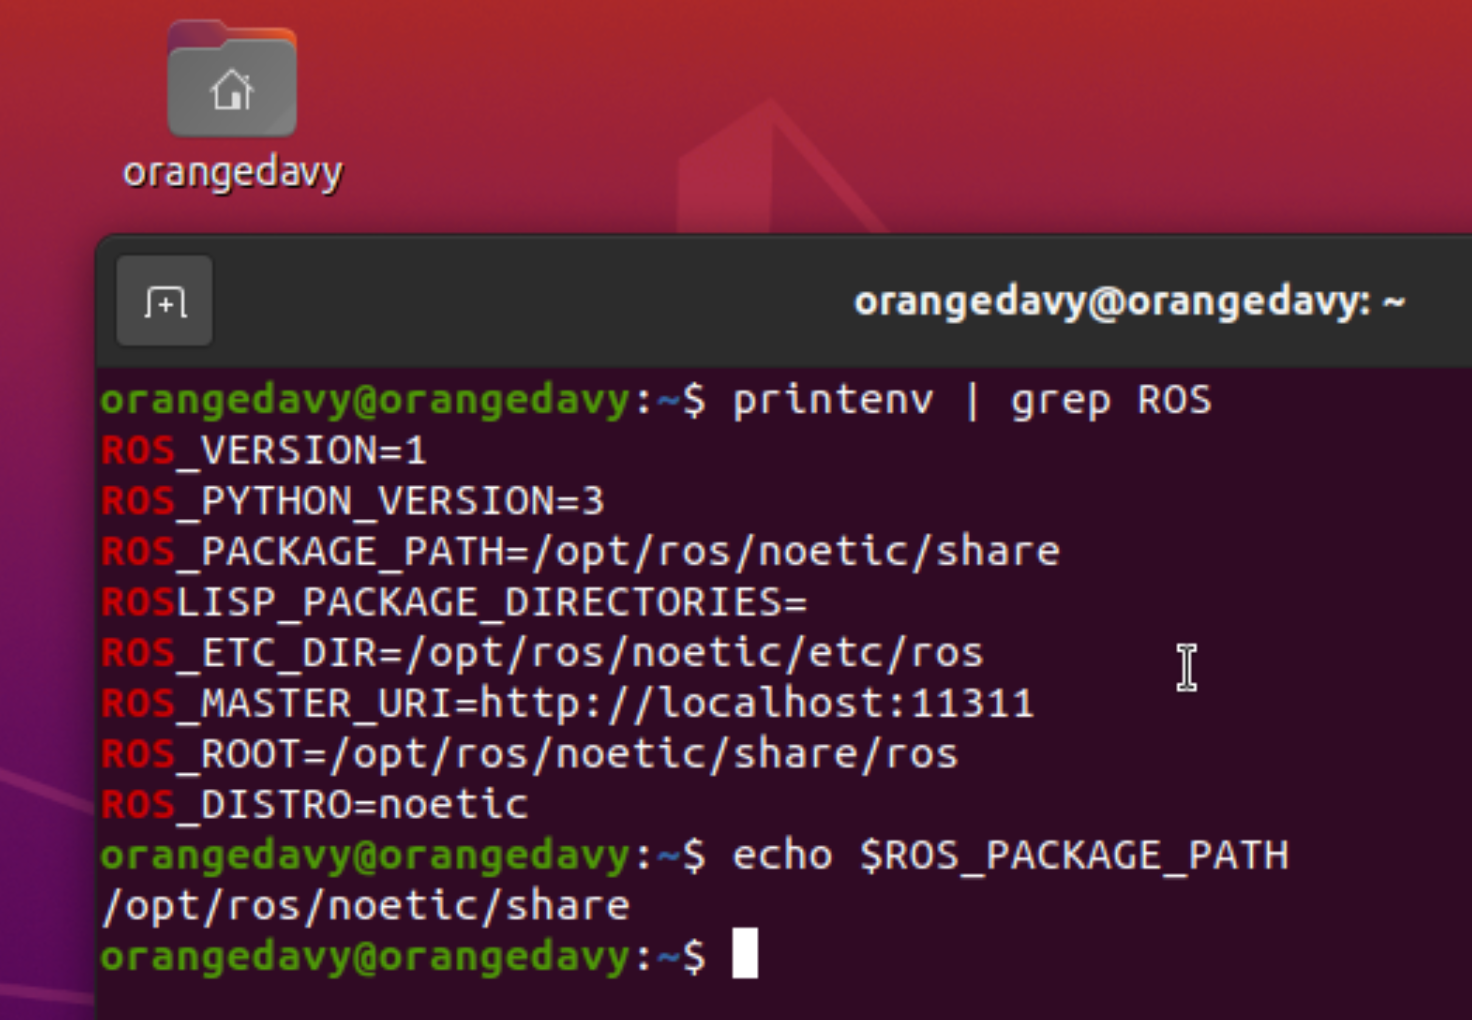
\includegraphics[width=14cm]{images/ros_package_path.png}\vspace{-10pt}
\caption{Printing \mintinline{bash}{$ROS_PACKAGE_PATH}.}\label{fig:ros_package_path}
\end{figure}


\subsection {Navigating the ROS Filesystem}

After soucing the setup.bash in your workspacex, please take a screen-shot of you using \textbf{rospack}, \textbf{roscd} and \textbf{rosls} and their results.Your screenshot is shown below: 

\begin{figure}[H]
  \centering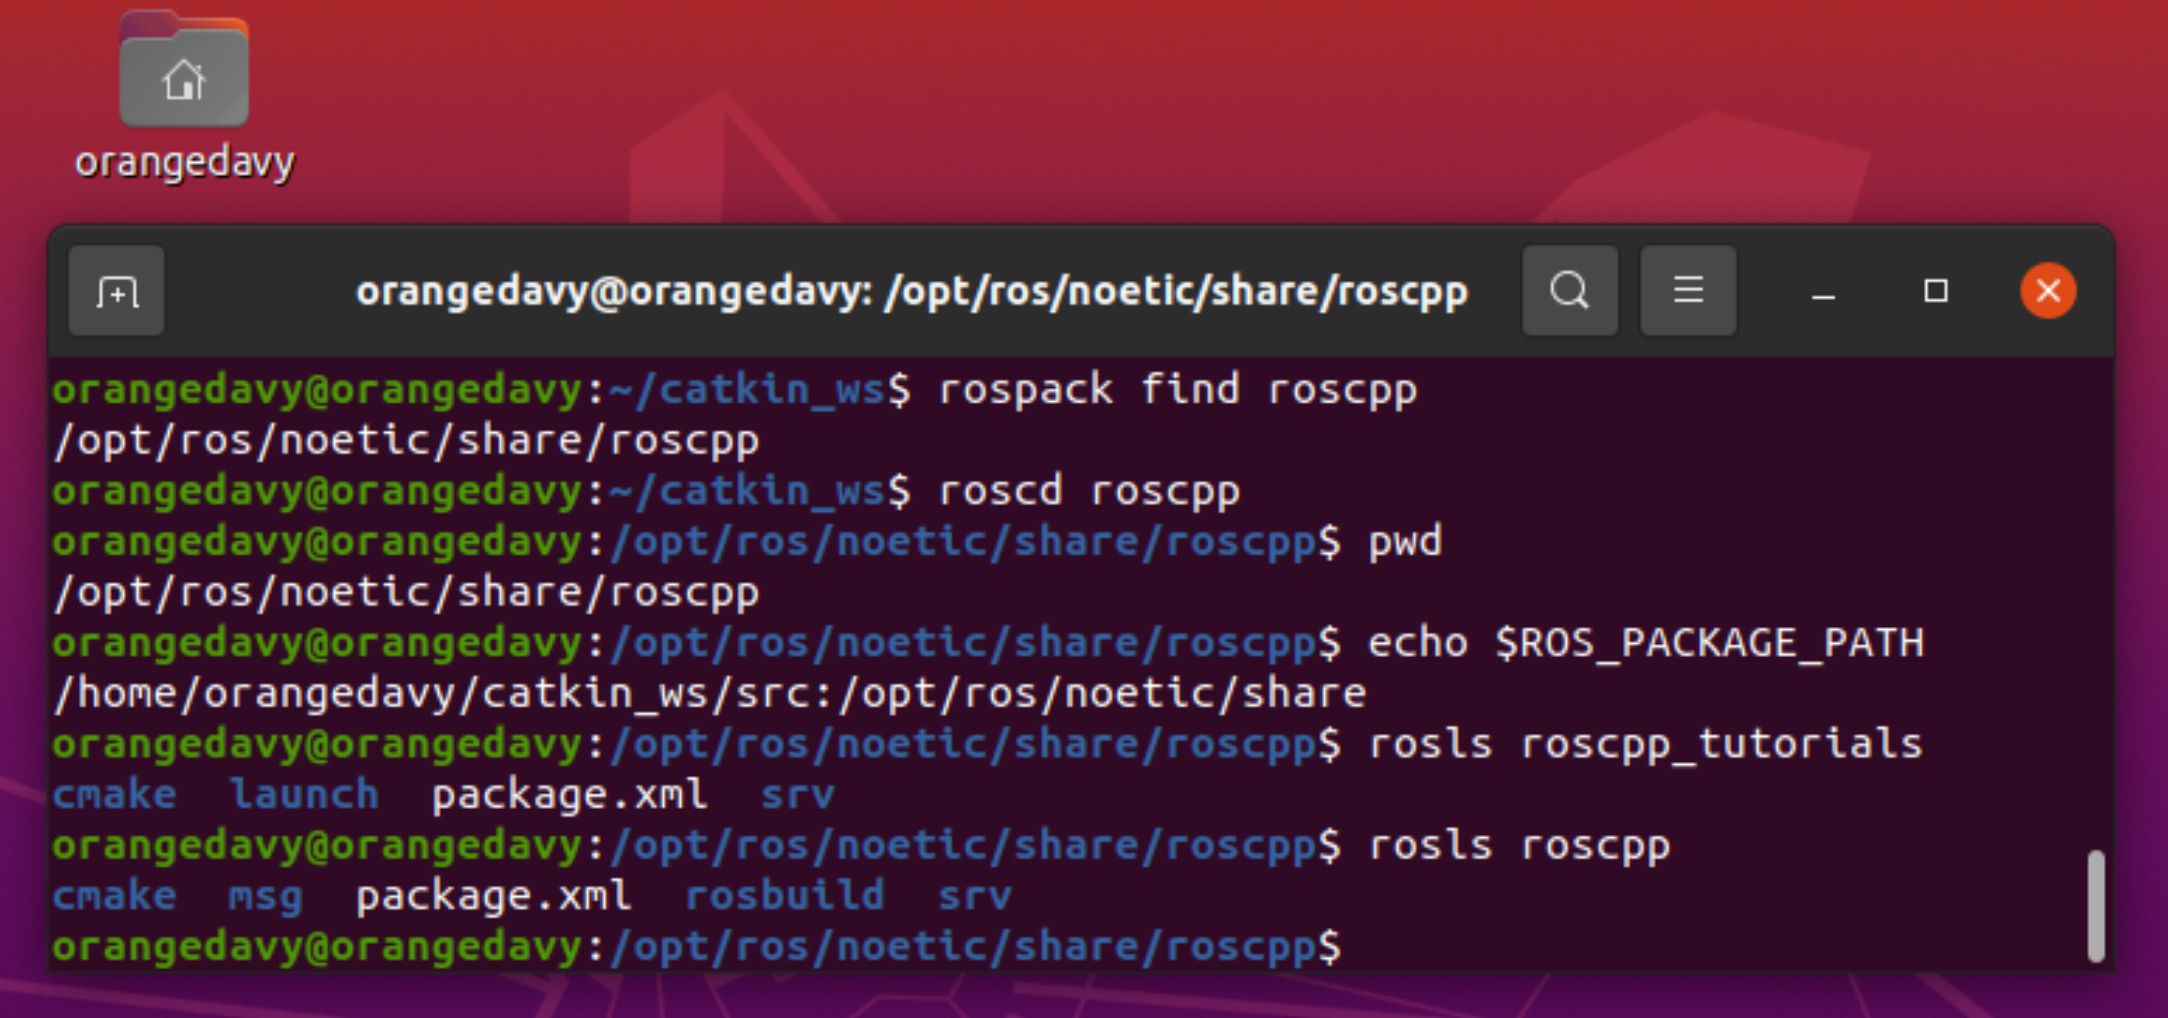
\includegraphics[width=14cm]{images/rospack_roscd_rosls.png}\vspace{-10pt}
  \caption{Using \mintinline{bash}{rospack, roscd, rosls}.}\label{fig:rospack_roscd_rosls}
  \end{figure}


\subsection{Creating and Building a ROS package}
Following tutorial 3 and 4, please provide a screenshot of the list of files in the src folder in the catkin workspace:

\begin{figure}[H]
  \centering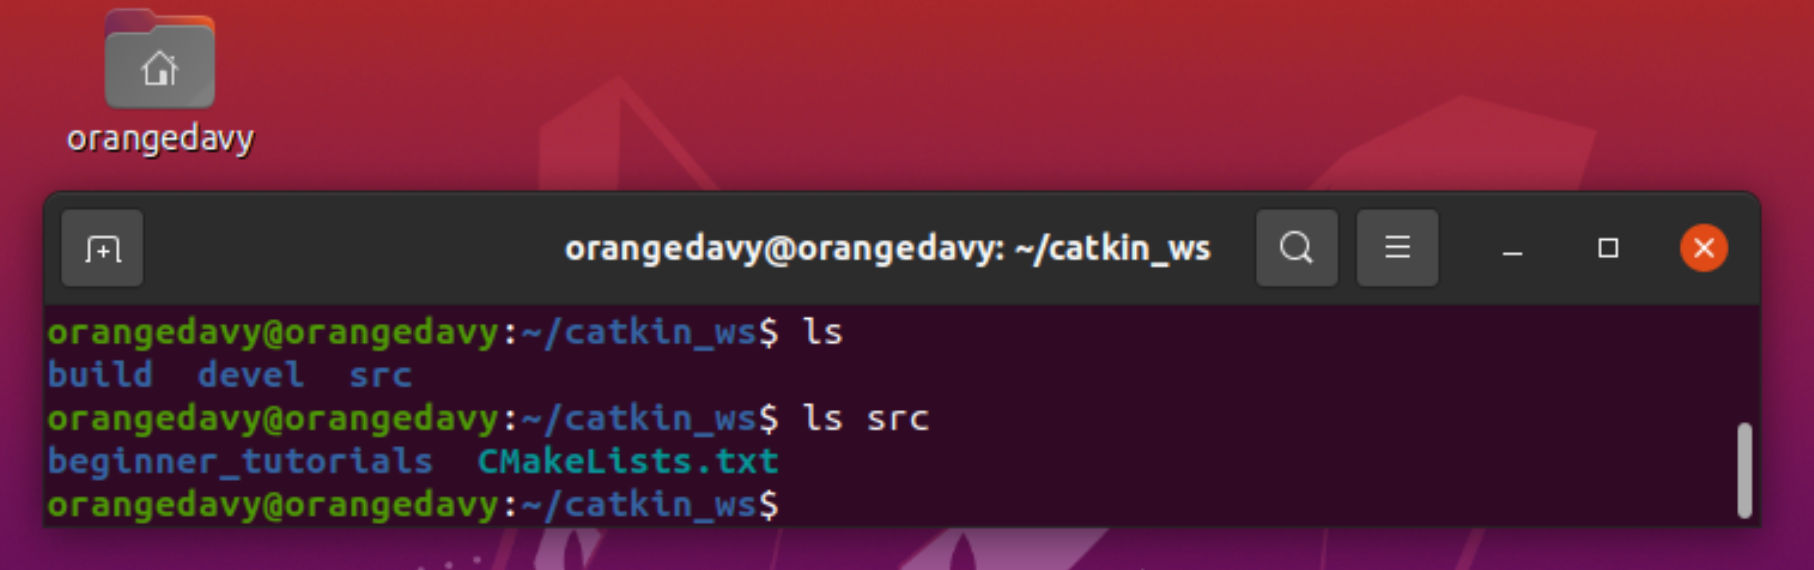
\includegraphics[width=14cm]{images/catkin_ws_src.png}\vspace{-10pt}
  \caption{Checking \mintinline{bash}{src} folder in catkin workspace.}\label{fig:catkin_ws_src}
  \end{figure}


\subsection{Understanding ROS Nodes}
Please answer the following questions:
\begin{enumerate}
\item How to run the ROS master. 

Solution:

\begin{minted}{bash}
  $ roscore
\end{minted}

\item How to run the turtlesim\_node.

Solution:

\begin{minted}{bash}
  $ rosrun turtlesim turtlesim_node
\end{minted}

\item How to check the list of running ROS nodes.

Solution:

\begin{minted}{bash}
  $ rosnode list
\end{minted}

\end{enumerate}

\subsection{Understanding ROS Topics}
\begin{enumerate}
    \item Use the node "turtlesim\_node" and "turtle\_teleop\_key" to draw a path of your choice and take a screenshot. Your screenshot is shown below:
    
    \begin{figure}[H]
      \centering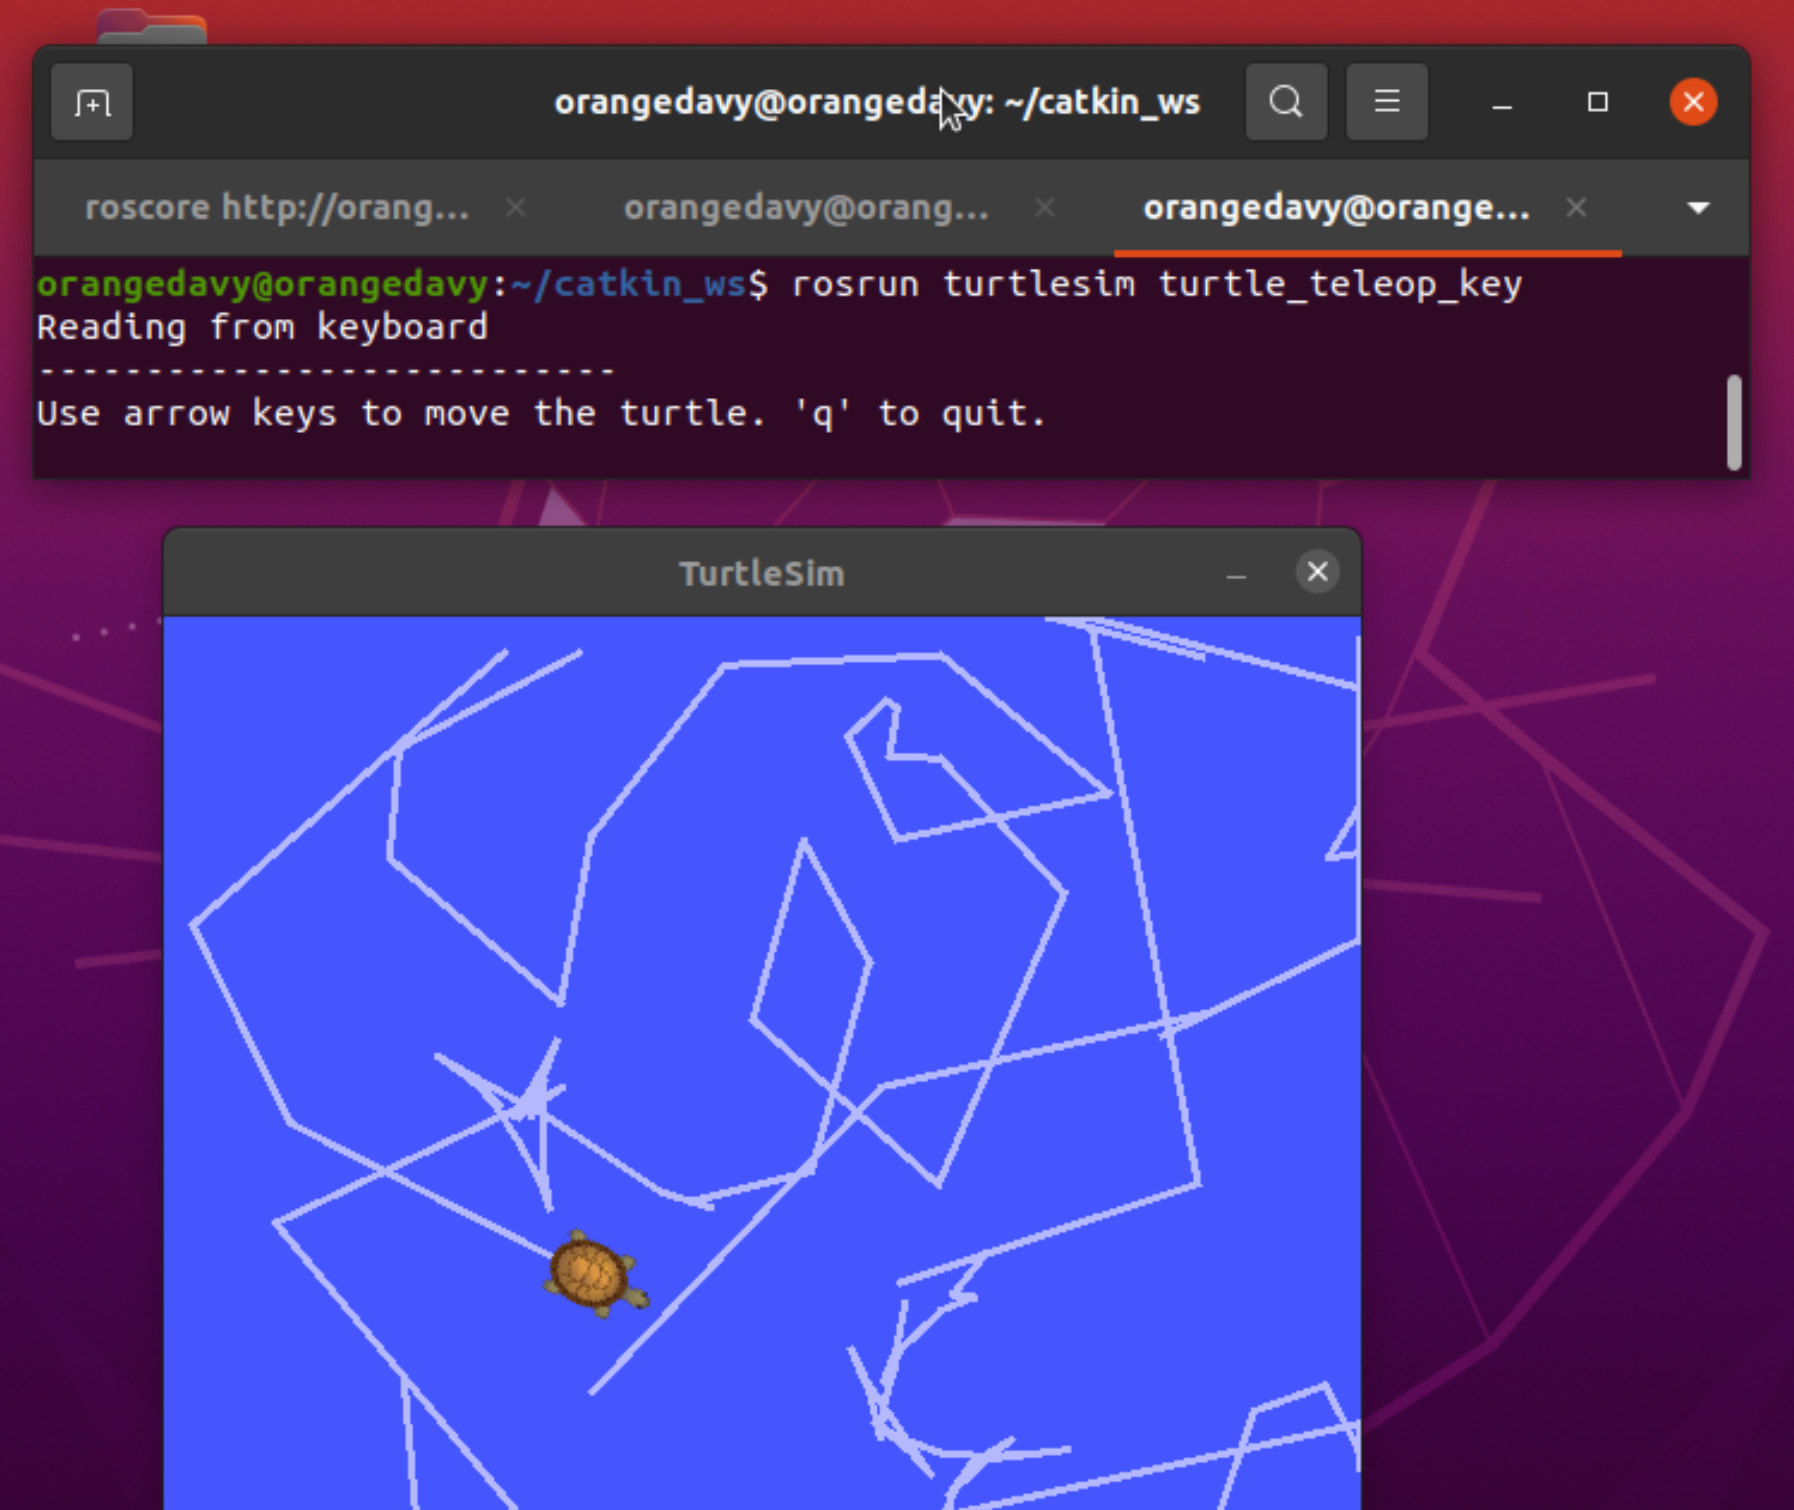
\includegraphics[width=14cm]{images/turtlesim_path.png}\vspace{-10pt}
      \caption{Drawing path with \mintinline{bash}{turtlesim_node} and \mintinline{bash}{turtle_teleop_key}.}\label{fig:turtlesim_path}
      \end{figure}
    

    \item Please briefly explain what is ROS topic, what is ROS message, their relationship and how to check the type of topic.
    \begin{enumerate}
      \setlength{\parskip}{1em}
      \item\textbf{ROS topic}: ROS topic transports information between nodes. The information is organized as a data structure and can have different data types. Topics can be identified by their name and their type.
      \item\textbf{ROS message}: ROS message is the information sent by the topic between nodes. To communicate, the publisher and subscriber need the same type of message, which defines the type of its topic.
      \item\textbf{Check type}: \mintinline{bash}{$ rostopic type [topic]}
    
    \end{enumerate}

\end{enumerate}

\subsection{Understanding ROS Services and Parameters}
\begin{enumerate}
\item Use the spawn service in turtlesim\_node to create a new turtle at \textbf{(x,y) = 2, 3; theta = 0.5; name = "turtleNo2"} and take a screenshot of TurtleSim window:

\begin{figure}[H]
  \centering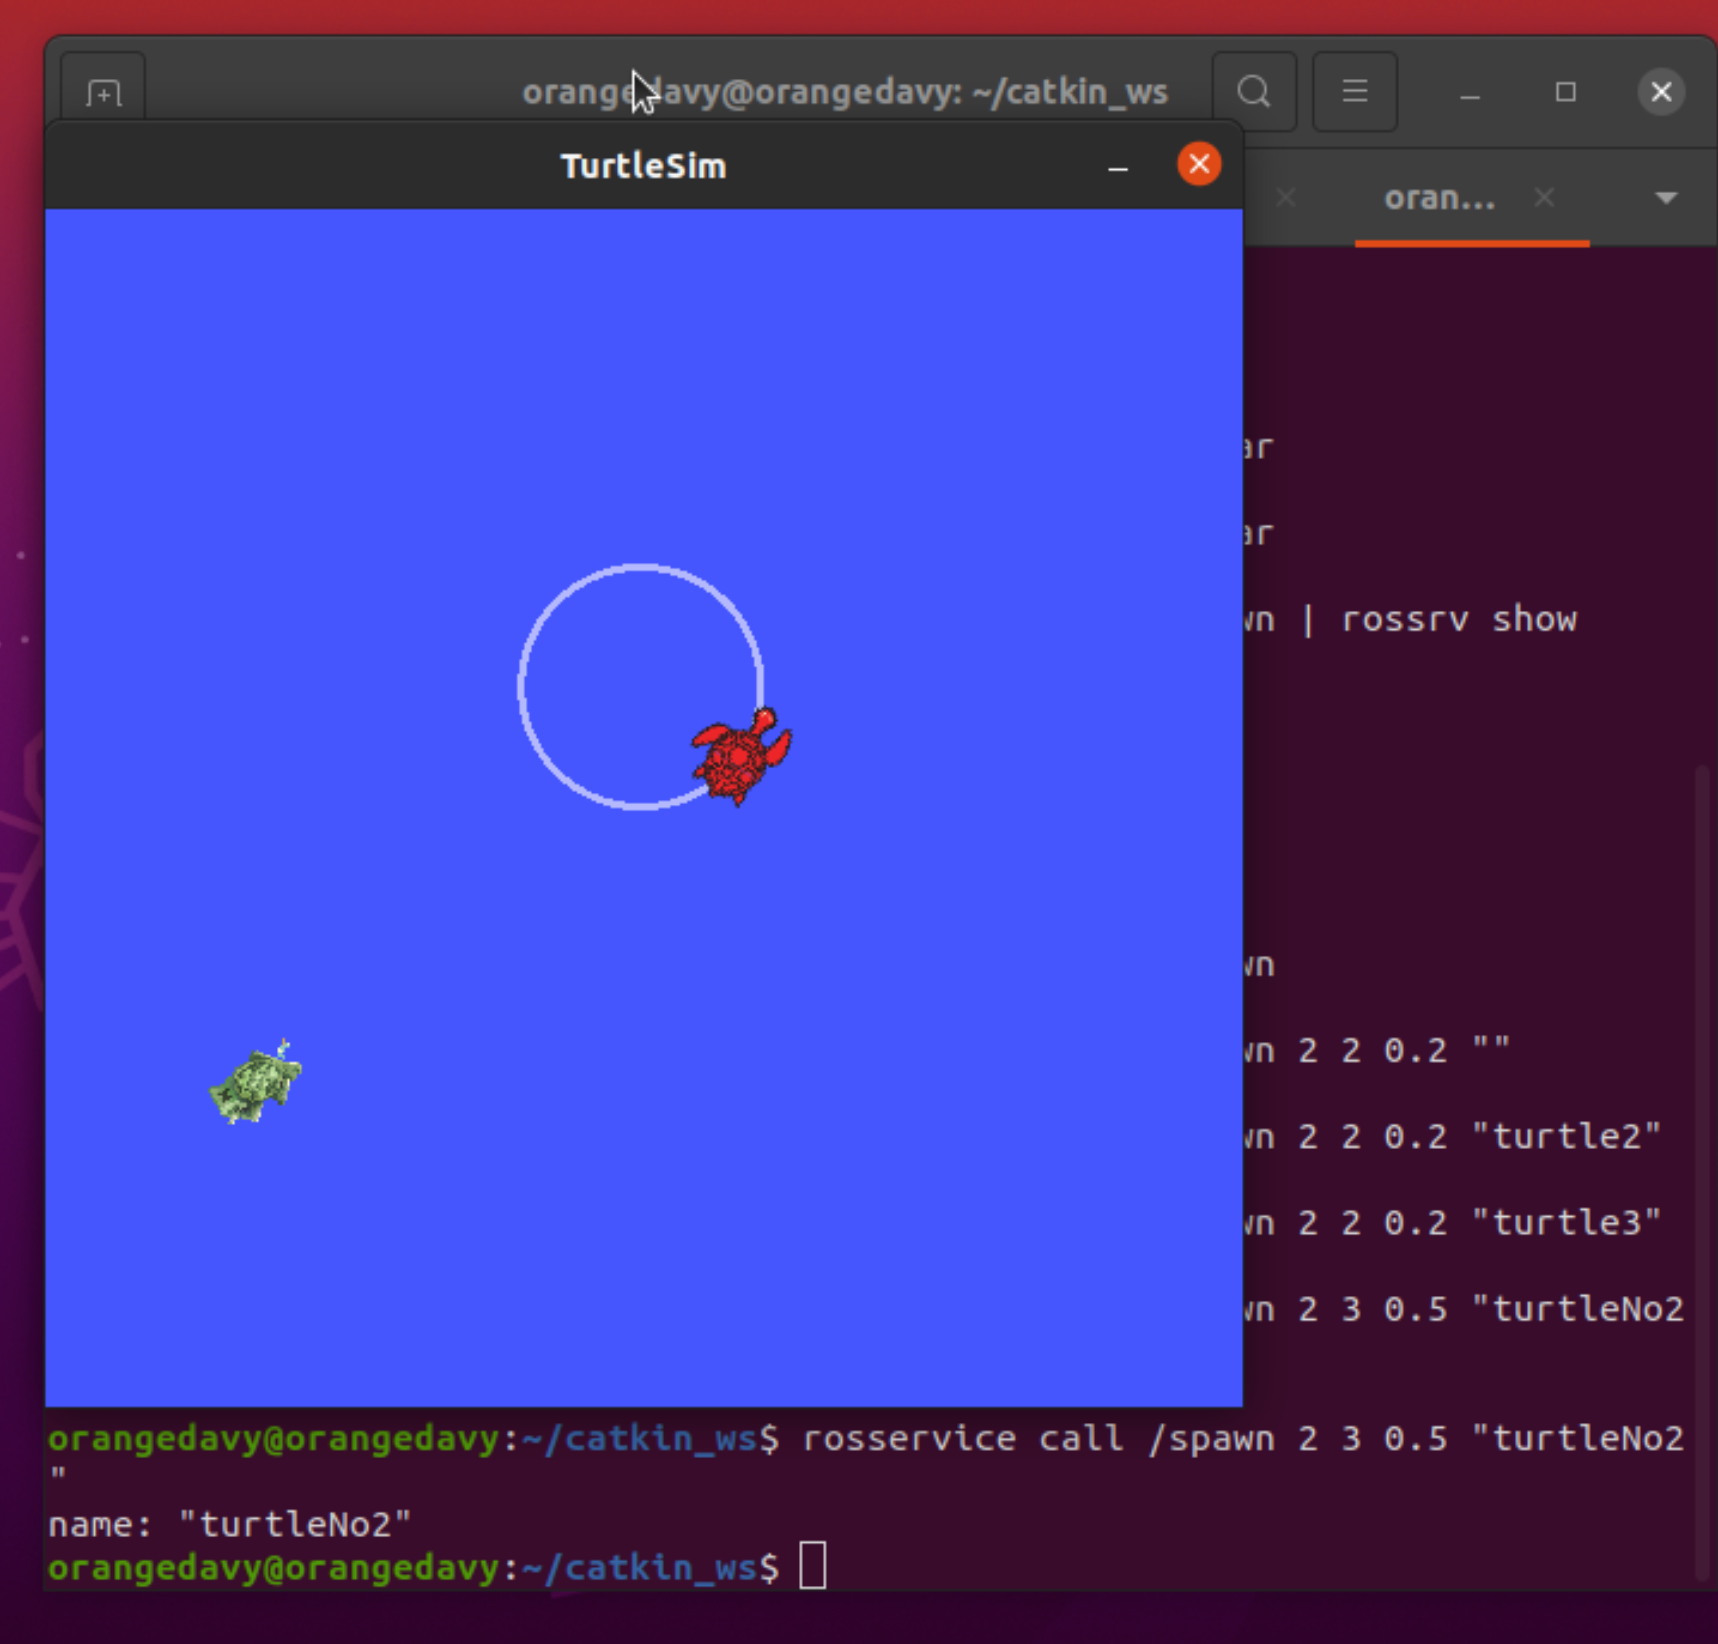
\includegraphics[width=14cm]{images/turtle_no_2.png}\vspace{-10pt}
  \caption{Spawning the new \mintinline{bash}{turtleNo2} instance.}\label{fig:turtle_no_2}
  \end{figure}


\item Figure out how to use the /kill service and use it to remove the turtle you created in the question 1. Please write down the command:

\begin{minted}{bash}
  $ rosservice call /kill "name:'turtleNo2'"
\end{minted}

\end{enumerate}

\subsection{Using roslaunch}
There is an example launch file in the Lab0.zip. Check the content and roslaunch it. Please explain what does the launch file do? What are the benefits of using launch files/roslaunch?

\setlength{\parskip}{1em}
\textbf{Command}: \mintinline{bash}{$ roslaunch example.launch}

\textbf{Explanation}: The example launch file creates a new turtle named \mintinline{bash}{turtlesim_node} with a node in the package \mintinline{bash}{turtlesim}, while enables another that allows the user to
move the turtle around with arrow keys under the name \mintinline{bash}{turtle_teleop_key}.

\textbf{Benefits}: Using launch files is a tidy way for the user to initiate several nodes with desired configurations and parameters all at once.


\subsection{Creating a ROS msg and srv}
As we have learned ROS messages and ROS services, here we will learn how to write customized messages and services. 
\begin{enumerate}
    \item Please follow the tutorial to create a msg file named Num in the beginner\_tutorials package. Modify the package.xml and CMakeLists.txt, and provide a screenshot of the result of 
\begin{minted}{bash}
  $ rosmsg show Num
\end{minted}

\begin{figure}[H]
  \centering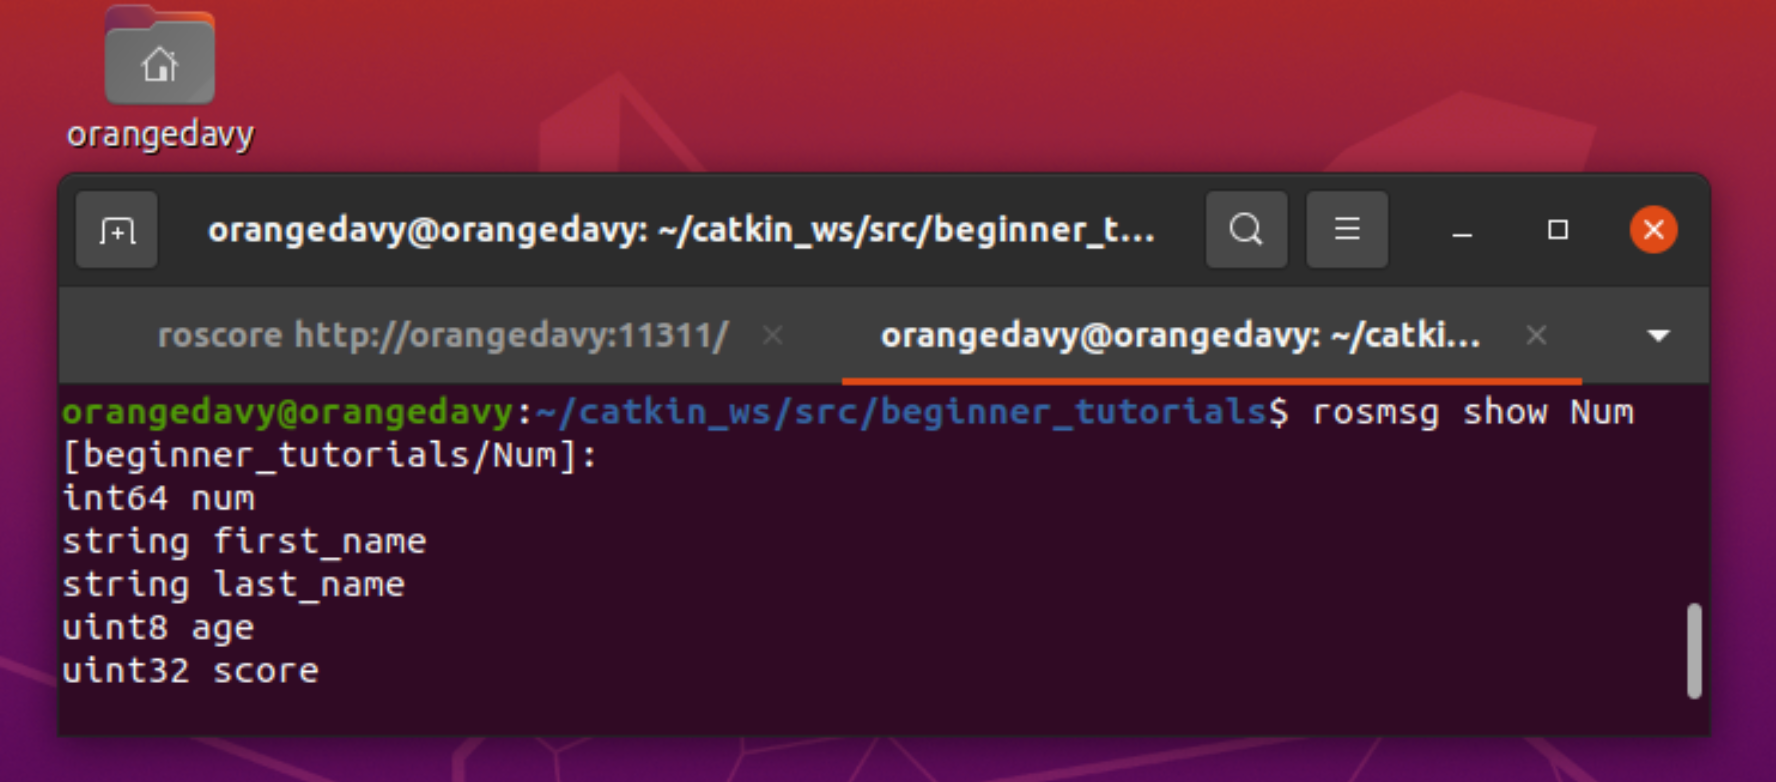
\includegraphics[width=14cm]{images/rosmsg_show_num.png}\vspace{-10pt}
  \caption{Creating a \mintinline{bash}{msg} file \mintinline{bash}{Num}.}\label{fig:rosmsg_show_num}
  \end{figure}

    \item Follow the tutorial to create a srv named AddTwoInts in beginner\_tutorials. Then provide a screenshot of the result of 
\begin{minted}{bash}
  $ rossrv show beginner_tutorials/AddTwoInts
\end{minted} 

\begin{figure}[H]
  \centering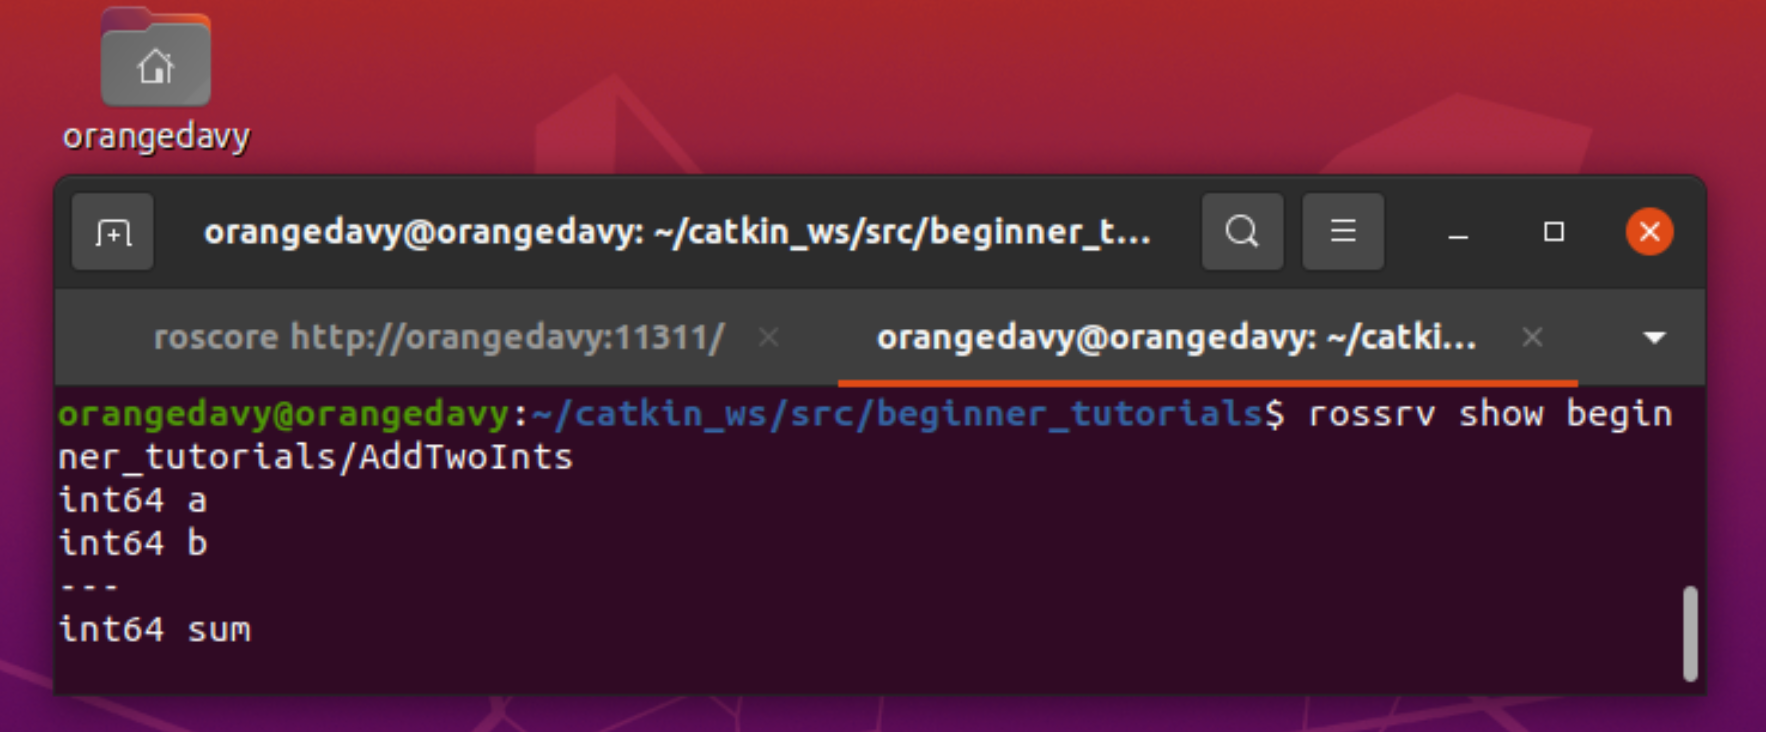
\includegraphics[width=14cm]{images/rossrv_show_ATI.png}\vspace{-10pt}
  \caption{Creating a \mintinline{bash}{srv} file \mintinline{bash}{AddTwoInts}.}\label{fig:rossrv_show_ATI}
  \end{figure}

\end{enumerate}


\subsection{Writing a Simple Publisher and Subscriber (Python)}
Please briefly explain what does the sample codes do? What are the names of the publisher and subscriber nodes? What's name of the topic? What's the topic type?

\setlength{\parskip}{1em}
\textbf{Explanation}: The sample codes are divided into a Publisher and a Subscriber. The former creates a publisher nodes that publishes to a certain topic a certain type of message at a desired rate until it stops.
The latter utilizes the callback mechanism to subscribe to the messages published to the topic as it works.

\textbf{Nodes}: Publisher name: \mintinline{bash}{talker}, Subscriber name: \mintinline{bash}{listener}.

\textbf{Topic}: Topic is named \mintinline{bash}{chatter}, of the type \mintinline{bash}{std_msgs.msgs.String}.

\subsection{Examining the Simple Publisher and Subscriber}
After running the two nodes, let's do one more step. Open a new window, echo the topic that is published/subscribed by the nodes and take a screenshot:

\begin{figure}[H]
  \centering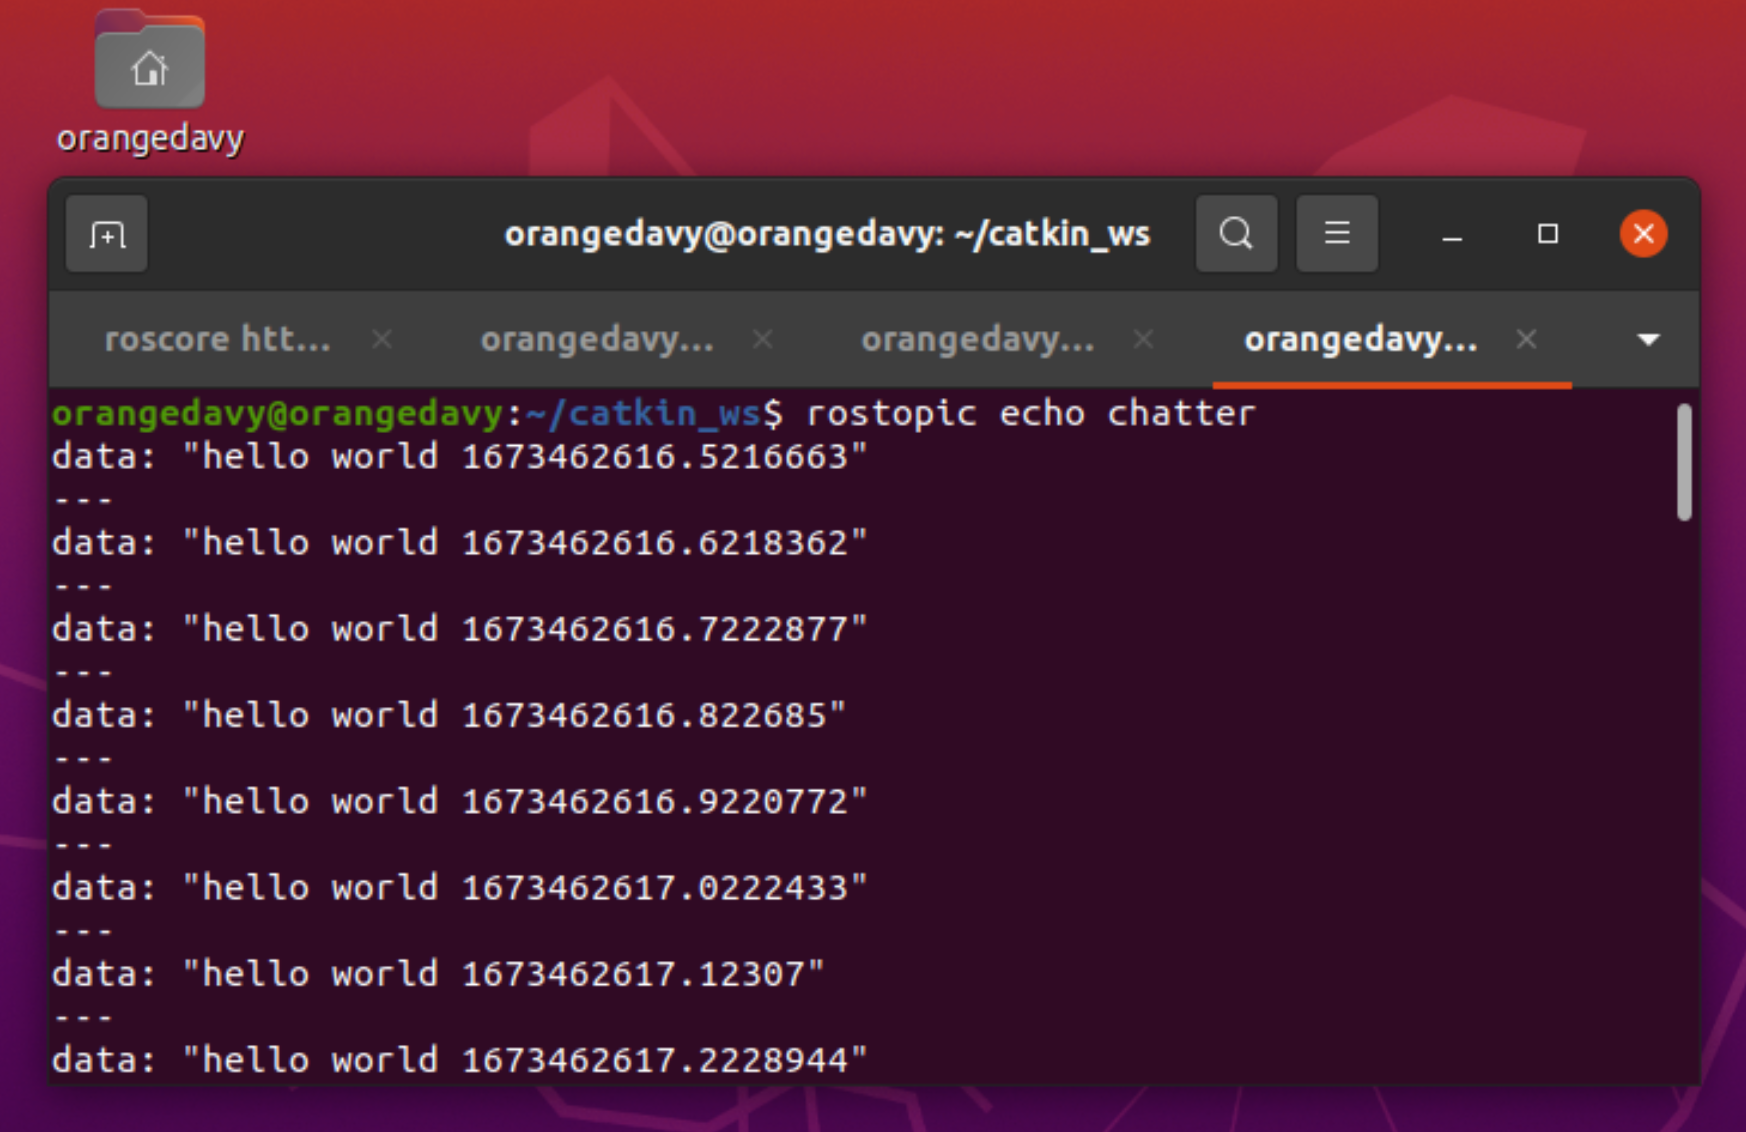
\includegraphics[width=14cm]{images/rostopic_echo_chatter.png}\vspace{-10pt}
  \caption{Echoing the messages published to \mintinline{bash}{chatter}.}\label{fig:rostopic_echo_chatter}
  \end{figure}

\subsection{Writing a Simple Service and Client (Python)}
What's name of the service? What's the service type?

\textbf{Service}: Service name is \mintinline{bash}{add_two_ints}, of the type \mintinline{bash}{AddTwoInts}.

\subsection{Examining the Simple Service and Client}
After finishing the tutorial, you will have an idea about how the server and client works. When you write your own service, you may want to examine that your service runs properly before writing the client. As the add\_two\_ints\_server is running, try to examine that service runs as expected using 2 plus 3 as a test case and take a screenshot. (Hint: use rosservice)

\begin{figure}[H]
  \centering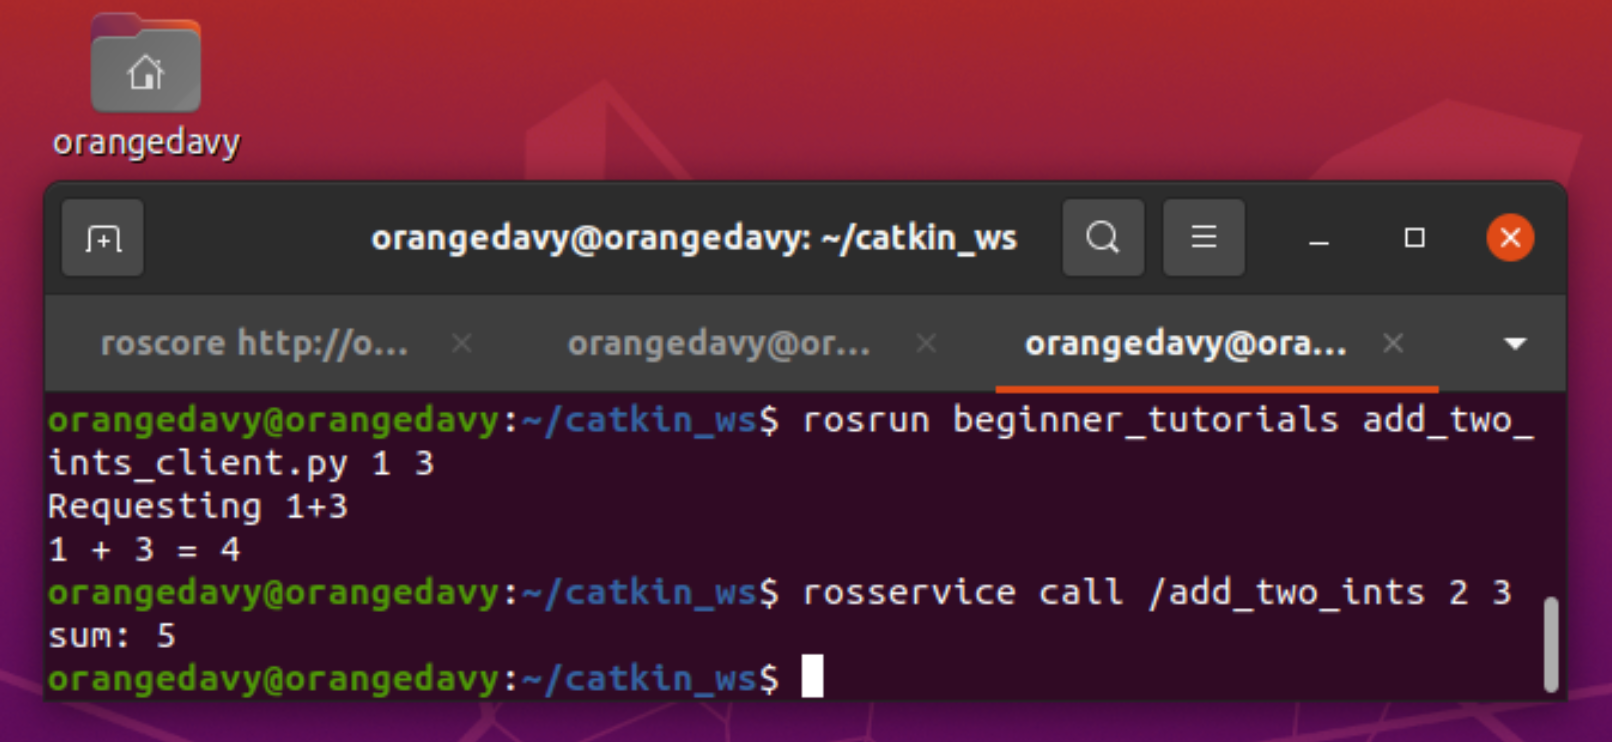
\includegraphics[width=14cm]{images/add_two_ints.png}\vspace{-10pt}
  \caption{Testing the service with \mintinline{bash}{2 + 3}.}\label{fig:add_two_ints}
  \end{figure}

\subsection{Recording and playing back data}
Follow the tutorial 17, record data of all topics for around 10 seconds. After this step, please take a screenshot of the info of your recorded bag file:

\begin{figure}[H]
  \centering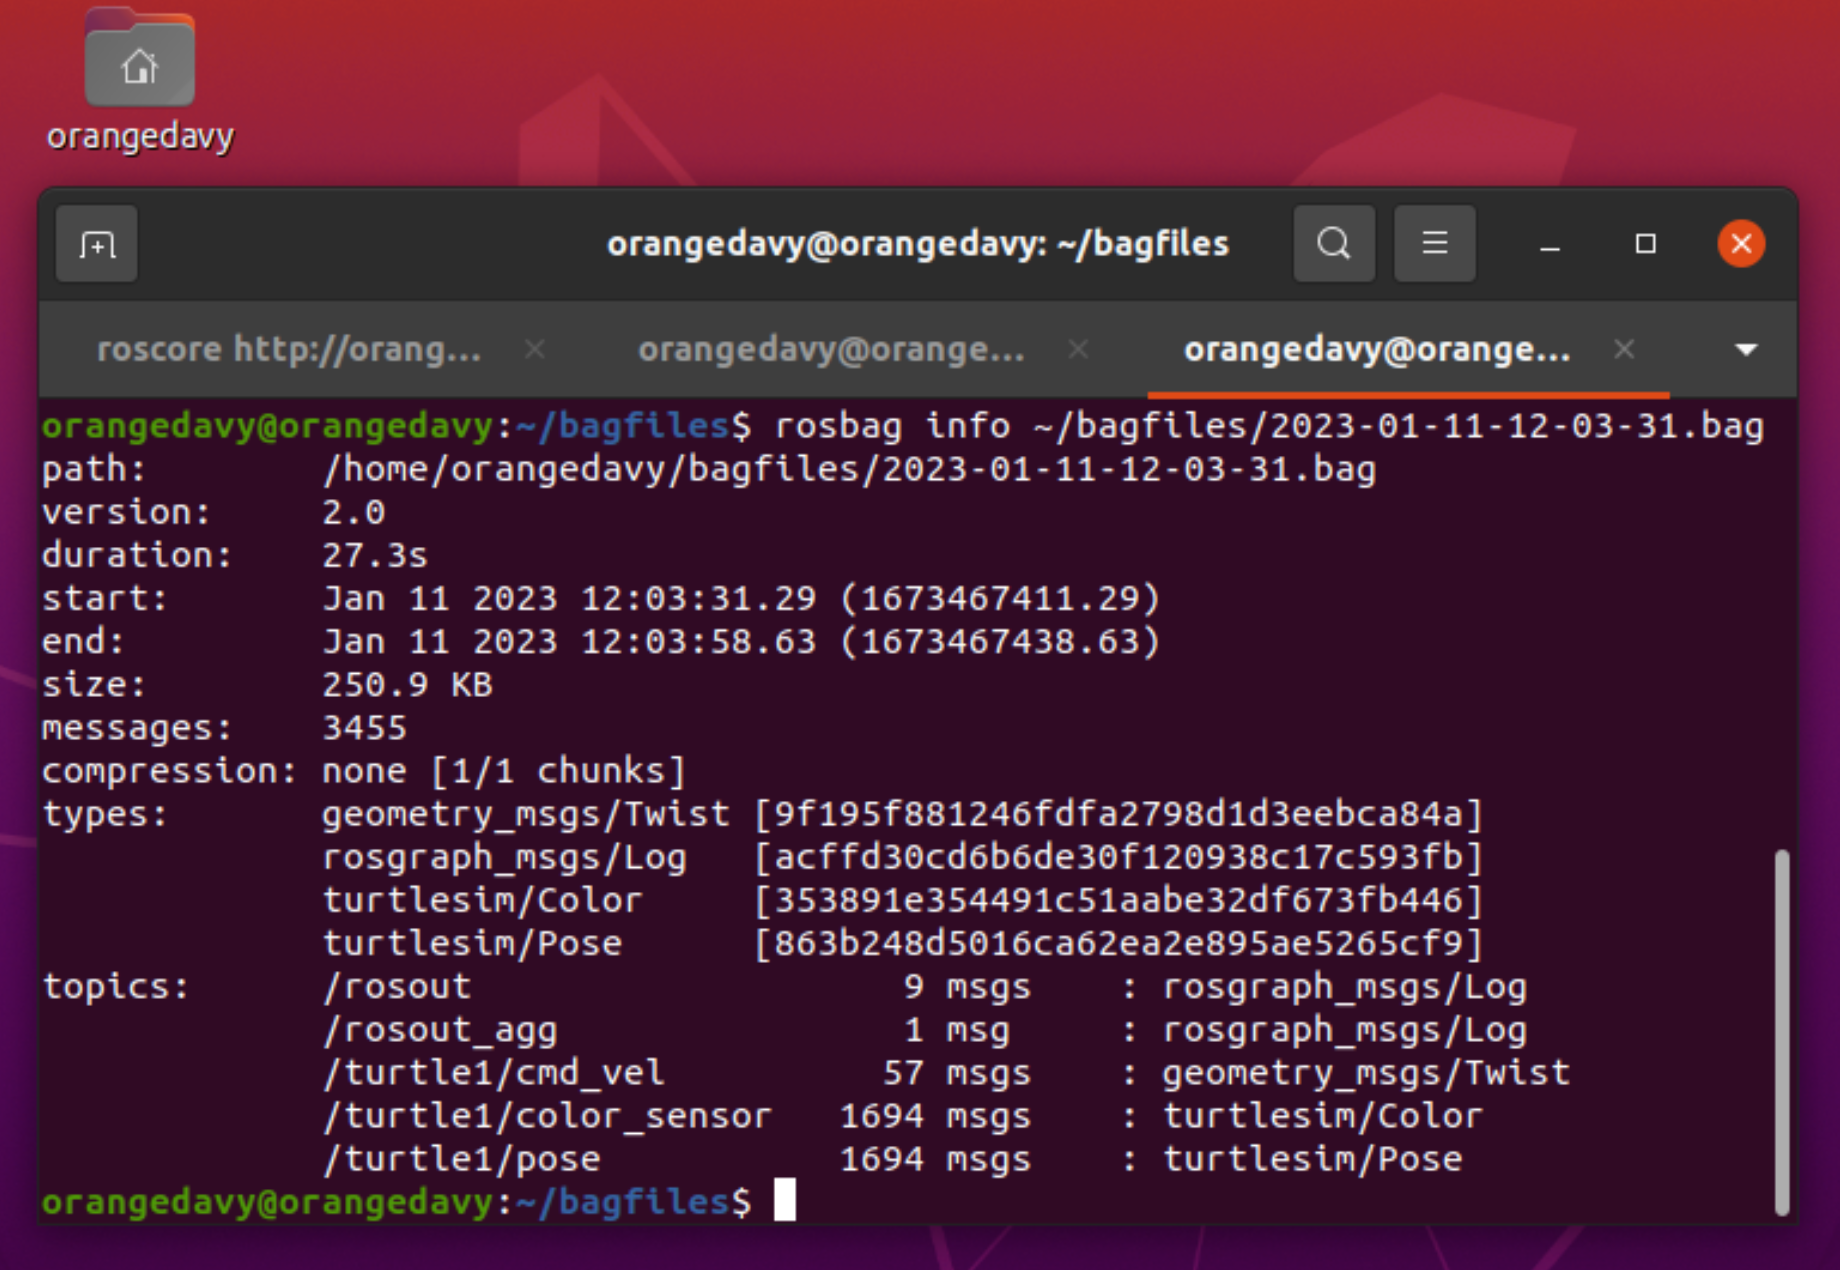
\includegraphics[width=14cm]{images/rosbag_info.png}\vspace{-10pt}
  \caption{Recording bag files with \mintinline{bash}{rosbag info}.}\label{fig:rosbag_info}
  \end{figure}

\end{document}